\documentclass[12pt,a4paper]{article}
\usepackage[utf8]{inputenc}
\usepackage{amsmath}
\usepackage{amsfonts}
\usepackage{amssymb}
\usepackage[left=2cm,right=2cm,top=2cm,bottom=2cm]{geometry}
\usepackage{graphicx}
\usepackage{float}
\usepackage{wrapfig}
\usepackage{caption}
\usepackage{sidecap}
\usepackage{subcaption}
\usepackage{tabulary}
\usepackage{pdflscape}
\usepackage{afterpage}
\usepackage{capt-of}% or use the larger `caption` package
\usepackage[usenames, dvipsnames]{color}

\author{Kelian Dascher-Cousineau}
\title{Masters Thesis: The Evolution of Fault Slip Surfaces with Cumulative Displacement}


\begin{document}

\maketitle

\begin{abstract}

Fault slip surface roughness determines fault strength, friction and dynamic fault processes. Wear models and field observations suggest that roughness decreases with cumulative displacement. However, measurements have yet to isolate the effect of displacement from other possible controls, such as lithology or tectonic setting. We present an unprecedentedly large fault surface dataset collected in and around the San-Rafael Desert, S.E. Utah, United States. In the study area, faults accommodated regional extension at shallow 1 to 3 $km$ depth and are hosted in the massive, well sorted, high porosity Navajo and Entrada sandstones. Existing detailed stratigraphic throw profile provide a maximum constraint for displacement. Where cross-sectional exposure is good, we measure exact displacement imparted on slip surfaces using offset in marker horizons. Thereby, we isolate for the effect of displacement during the embryonic stages of faulting (0 to 60 $m$ in displacement). Our field observations indicate a clear compositional and morphological progression from isolated joints or deformation bands towards smooth, continuous and mirror-like fault slip surfaces with increasing displacement. To quantify these observations, slip surfaces were scanned with a white light interferometer, a laser scanner and a ground based Lidar. Together these instruments resolve more than eight decades of spatial bandwidth (from less than $\mu m$'s to $m$'s in scale). Preliminary results indicate that roughness decreases with displacement according to a power law. Roughness measurement associated with only maximum constraints on displacements corroborate this result—for a given displacement, minimum roughness is bounded by the later smoothing trend. In addition, we find that the maximum roughness is fixed—bounded a by a primordial roughness corresponding to that of joints surfaces and deformation band edges. Our results build towards a coherent model of fault wear robust to ambiguities associated to displacement estimates, spatial scaling and geological context.

\textcolor{red}{\textit{Will have to include relationship to white light data, modelling results/interp}}

\end{abstract}

\section{Introduction}

\textcolor{red}{\textit{
Would closely follow my project proposal:}}

\subsection{Motivation}

Faults are a characteristic feature of the Earth’s brittle crust. Fluid flow, seismicity and crustal mineralization are just few systems upon which faults act as major controls (Sibson, 1977). In spite of their importance, some aspects of faults and their underlying processes remain poorly understood. How strong is a fault? How do faults mature? Are small faults mechanically different to large faults? Fault geometry has been shown to be a key parameter controlling the mechanical behavior and evolution of faults (e.g. Lay et al., 1982; Aki, 1984; Power et al. 1988; Chester and Chester, 2000), but these questions are not yet fully answered.

Slip on a fault occurs on discrete slip surfaces in fault zones (Davatzes and Aydin, 2005). These surfaces are not planar; they are rough. Roughness is observable at all scales (Scholtz and Aviles, 1986; Candela et al., 2012). Slickenlines, corrugations, mullions and jogs are all  surface features that can be seen at different length scales (Sagy and Brodsky, 2009). Field studies have found common characteristics in the topography of fault surfaces. These can be summarized as follows: 1) Fault surfaces appear to be well defined by large fractal domains, wherein 2) faults are smoother at larger length scales (Scholtz and Aviles, 1986; Candela et al., 2012), 3) rougher in the slip perpendicular direction than in the slip parallel direction (Lee and Bruhn, 19960, and 4) slip surfaces are smoother with cumulative displacement (Sagy et al., 2007). Fault roughness has been demonstrated to be critical in determining the strength (Chester and Chester, 2000, Brodsky et al., 2016), triggering (Parsons, 2008), dynamic properties (Candela et al., 2011; Dunham et al., 2011), spatial distribution (Parson, 2008) and failure recurrence of faults (Stirling et al., 1996). It is increasingly evident that roughness is a fingerprint of fundamental features of the faulting process (Brodsky et al., 2016). In accordance, incorporating more complex sources geometries has become a more frequent practice in dynamic earthquake rupture modelling (Shi and Day, 2013; Dunham et al., 2011). 

Changes in roughness, as determined by cumulative displacement (Sagy et al, 2007; Brodsky et al, 2011), imply faults mature. Fundamental differences between immature and mature fault have far-reaching implications. Fixed source parameter scaling of earthquakes is a pillar of earthquake seismology. However, analysis of seismic signals of immature faults vs. mature faults suggest that scaling is sensitive to cumulative displacement. This observation leads to an interpretation of fundamental differences in earthquake populations. Specifically fault maturation would undermine the applicability of a constant magnitude scaling. Evolving mechanical properties such as fault friction and static strength—both associated to fault roughness—would imply that immature and mature faults belong to distinct populations with distinct scaling. (Harrignton and Brodsky, 2011)

While there has been significant progress in understanding the role of roughness in the faulting process, how and why fault surfaces change is still unclear (e.g. Candela et al., 2011; Dunham et al., 2011; Brodsky et al., 2016). Sagy et al. (2007) noted a systematic decrease in roughness of ‘mature’, large displacement faults compared to ‘immature’ faults with low displacements. Similar results have since been observed along reactivated joints, in laboratory experiments (Davidesko et al., 2014), and in compilations of fault roughness analysis (Brodsky et al., 2011; Candela et al., 2012). These studies all attribute the decrease in roughness to wear at the fault interface. However, these data show only weak correlations between fault roughness and cumulative displacement. Indeed, relating roughness and cumulative displacement is not trivial. Fault surfaces in exhumed faults are rarely well preserved. Furthermore, obtaining well-constrained displacement estimates is contingent on the presence of precise and accurate kinematic indicators. Combining observations over a broad range of displacements is challenging. Consequently, it is unclear whether trends observed in compilations of roughness measurements from multiple faults are directly attributable to displacement or a combination other geological factors. For instance, while comparing fault surfaces from geologically diverse datasets, variations in lithology, faulting mechanism, temperature and depth may all be introducing further systematic variations. 

Additionally, the evolution of roughness represents a novel insight into the architecture of a fault zone.  The geometry of the fault surface modulates the architecture of the whole fault zone (Mitchell and Faulkner, 2009). Changes in roughness require interaction between the slip surfaces and its direct surrounding (fault core), resulting in the formation of fault rock (Power and Tullis, 1988). In addition to earthquake mechanics, the architecture of a fault zone, and its corresponding permeability structure, is very important for hydrocarbon exploration (Shipton and Cowie, 2003). However, because the change in roughness by wear is poorly understood, the equivalent production of wear material, the fault rock, is also poorly understood. Fault rock thickness growth with displacement is documented (Sholtz, 1987), but variability is such that even order of magnitude estimates of thickness for a given displacement are unavailable.

	The objective of this project is to identify how and why fault surfaces change. In line with previous studies, I hypothesize that wear is a dominant mechanism in the evolution of fault surfaces with cumulative displacement. I will measure the surface roughness of natural fault surfaces with varying displacements to confirm and better quantify the role of cumulative displacement on fault roughness. This study will be broadly composed of the following three components: 1) data collection, 2) data processing and analysis and 3) interpretation of the results. Field work in Southern Utah will be conducted with the specific intent of collecting scans of pristine fault  surfaces with terrestrial laser scanners and hand-samples for laboratory high resolution scans. The roughness of the surfaces will then be quantified and related to corresponding displacement. A robust quantitative correlation between roughness and cumulative displacement will enable parameterized interpretation and modelling of the mechanics of fault wear. Based on my results, I will explore the mechanical implications of a changing fault surface as coupled to the fault zone. In this proposal, I first present the geological background and important concepts. I then follow by outlining the projected scientific method, data analysis and interpretation. I conclude with a time line for the completion of my thesis in a timely two year period. 

\subsection{Geology}

Field work will be conducted in the San-Rafael Desert, Utah (see figure 1). The San Rafael Desert hosts a sequence of gently dipping marine and sub-areal sedimentary rocks deposited from the Pennsylvanian to the Jurassic (see Figure 2). 
The San Rafael Desert is part of the San Rafael Swell, a monocline that formed when these sediments were uplifted as a passive drape fold above a reactivated basement reverse fault during the Late Cretaceous Laramide Orogeny (Kelly, 1955; Vrolijk et al., 2005). The swell is part of the broader Colorado Plateau (Kelly, 1955). Networks of joints and normal faults associated to further Laramide activity cross-cut sedimentary sequence accommodating North-South extension (Aydin and Johnson, 1978; Vrolijk et al., 2005). Specifically, within the San Rafael Swell we have selected the following field locations: 1) the Chimney Rock Fault Array, 2) the Big Hole fault and 3) a network of deformation bands in the Entrada formation near Goblin Valley State Park.  Advantages of theses field locations are manifold. First, the nearly pure quartzite lithology, extensional tectonic regime, depth (2-4 km or 40-80 MPa), temperature (estimates range from 45-90 oC) of activity, and faulting mechanism are all relatively consistent (Vrolijk et al., 2005). Consistency in these parameters is key to isolating the effect of displacement on the fault roughness. Moreover, both field locations exhibit well preserved fault surfaces that are exposed and accessible (see Figure 3). 
The Chimney Rock fault array is an orthorhombic set of faults that crops out at the northern end of the San Rafael Swell (Krantz, 1989, Davatzes et al., 2003). Two pairs of oppositely dipping normal faults crop out at the surface with preserved fault scarps. WNW-striking faults are interpreted to have formed by shear reactivation of joints, whereas ENE-striking faults initially formed from deformation bands (Davatzes, 2003). Exposure is very good, faults are abundant and have well preserved fault surfaces (Vrolijk et al., 2005). The Chimney fault array has studied to better understand of fault geometry (Shipton and Cowie, 2001; Shipton and Cowie, 2003), permeability (Shipton et al., 2002) and kinematics (Krantz, 1986; Krantz, 1989; Maerten et al., 2001; Davatzes et al., 2003) . As a result, detailed maps of the fault array have been produced (e.g. Maerten et al., 2001) . In addition, by using measurements of the separation between footwall and hanging wall cutoffs of sedimentary horizons, entire displacement profiles have been measured for faults with a wide range of displacements (Cowie and Shipton, 1998; Maerten et al., 2001; Shipton and Cowie 2001; Shipton and Cowie, 2003). 
The Big Hole fault is located just to the South-East of the Chimney Rock Fault Array. While not explicitly part of the fault array, the Big Hole fault shares a nearly identical geological setting. The Big Hole fault has been extensively studied in detail as an analog to hydrocarbon reservoir-scale faults. Displacements on the exposed fault range from 8 m to 39 m. (Shipton and Cowie, 2001; Shipton and Cowie, 2003) 
	Large networks of deformation band faults outcrop near Goblin Valley State Park on the southeastern margin of the San-Rafael Swell (Aydin and Johnson, 1978). Deformation bands are the result of concentrated shear deformation on narrow centimeter thick bands (Aydin and Johnson, 1978; Davatzes et al., 2003). Collapsing pore space accommodates this deformation. Deformation bands are interpreted as the embryonic stages of fault development (Fossen and Hesthammer, 1998; Fossen et al., 2007). Because deformation bands dramatically alter the local permeability structure, Goblin Valley has been extensively studied in light of fault nucleation and the implications for hydrocarbon circulation (e.g. Fossen et al., 2005; Tobari and Fossen 2009). At Goblin valley, arrays of deformation bands anastomose—outcropping as centimeter- to meter-sized slabs.  These are often bounded by discrete slip surfaces with well-preserved striations — i.e. roughness (Aydin and Johnson, 1978). Offsets in sedimentary beds have allowed previous studies to obtain detailed displacement measurements (e.g. Schultz and Fossen 2002). 
Together, these field locations offer the chance to survey well-preserved fault surfaces that have hosted displacements from embryonic stages to 30 m of displacement. Moreover, novel to this study, we will be able to survey multiple expressions of a single fault’s surface with various displacements according the displacement profile of the fault. 


\subsection{Fault Roughness}

The deviation from planarity formally defines roughness (Brown and Scholz, 1985). Pioneering studies used contact profilometers to measure the roughness of fault surfaces (Scholz and Aviles, 1986; Power and Tullis, 1991. Combined with surface profiles of large scale continental faults, faults were found to have a remarkably broad fractal band ranging over 10 orders of magnitude—from $10^{-5}$ to $10^5 m$ (Scholz and Aviles, 1986). Over these length scales, fractal scaling is said to be statistically self-affine. 	
A statistically self-affine profile along $x$ with heights $h(x)$, is invariant under the affine transformation:

\begin{equation}
\left\lbrace
  \begin{matrix}
   	x \rightarrow \lambda x \\
    h \rightarrow \mu h
  \end{matrix}
\right\rbrace
\end{equation}


This relation therefore implies an exponential relation between the scaling, $\lambda$ (along $x$), and $\mu$ (along $h$) such that:

\begin{equation}
\mu = \lambda^\varsigma
\end{equation}

Where $\varsigma$ is a constant named the Hurst exponent. Note that self-similarity, is an instance of self-affinity where the Hurst exponent is 1 (Schmittbulh et al., 1993). Developments in laser scanner technology over the past decade, particularly terrestrial laser scanners, allowed surfaces to be characterized by calculating the Hurst exponent from thousands of cross sectional profiles through a fault surface (e.g. Candela et al., 2012). Studies of natural mode I crack surfaces have observed self-affinity with a Hurst exponent of $\sim$0.8 at all scales of observation (Scholtz, 1985). Shear, or mode II cracks (i.e. faults) are different. They are anisotropic—the Hurst exponent parallel to shear ($\sim$0.6) is smaller than that in the shear-perpendicular direction ($\sim$0.8) (Lee and Bruhn, 1996). 

Another parameter is required to fully describe surface roughness. While the Hurst exponent describes the scaling behavior of the roughness it does not define the magnitude of the roughness. The pre-factor defines the amplitude of the scaling law (Candela et al., 2009). The pre-factor is subject to significant variation. Overall, observations show that fault surfaces have distinctly smoother profiles along slip direction than perpendicular to slip (Lee and Bruhn, 1996).
Many methods exist to quantify roughness scaling, possibly most intuitive of which is the Root Mean Squared ($RMS$) as a function of scale. For a profile of length $L$ with a point spacing of $\Delta x$ with deviation h from the best fit line, the $RMS$ for a given scale s is defined as follows:

\begin{equation}
RMS(s)=\sqrt{\dfrac{\Delta x}{L}\sum^{L/{\Delta x}}_{i=1} h^2_i}
\end{equation}


	The $RMS$ roughness of a fault or fracture exhibits power-law scaling with segment length. A self-affine profile should therefore plot as a straight line on a log-log plot of the $RMS$ as a function of the segment length with a slope equivalent to the Hurst exponent. (Schmittbuhl et al., 1993)
The power spectrum of a surface profile has been shown to yield more robust roughness metrics (Schmittbuhl et al., 1993; Candela et al., 2009). For a set of discretely sampled points, the power spectrum of a profiles is the result of a Fast Fourier Transform (FFT). The spectrum defines the surface profile as superposition of sinusoidal profiles.   In the frequency domain, rougher profiles will have correspondingly higher amplitudes, or power. The power spectrum, $P(k)$, of a self-affine profile (again in log-log space) defines a line as follows:

\begin{equation}
P(k) = Ck^{(-1-2\varsigma)}
\end{equation}

Where $k$ is the frequency and $C$ is the pre-factor (Candela et al., 2009). 

\subsection{The evolution of slip surfaces with displacement}

In this project, I hope to address how slip surfaces change. Many processes could cause the slip surface to change.   In fact, the cause of change to the slip surface is not uniquely recorded by the roughness. Fundamentally, a fault surface can only change according to the following mechanisms:
\begin{itemize}
	\item[] \textit{Addition of material}
	\item[] \textit{Redefinition of the slip surface by fracture}
	\item[] \textit{Removal of material}
\end{itemize}
	
I have hypothesized that the change in surface roughness is the result of wear—an instance of removal of material. As fault blocks slide past each other, frictional wear is an inevitable process. Layers of comminuted fault rock are direct evidence of this process (Power and Tuillis 1988). Wear is the subject of a vast field of research, particularly in engineering and tribology due to interest in lubricating and manufacturing machine parts for longevity (Meng and Ludema, 1995). Here, I outline only basic wear mechanics (i.e. Archard, 1953). Wear is formally defined as frictionally induced volume removal from surfaces in sliding contact. The wear rate, the amount of wear per unit distance is broadly related to the real area of contact and loading. When two surfaces are put in direct contact, the real area of contact is much smaller than the nominal surface areas because the load is supported at microscopic protrusions from a surface, called asperities. Remote loading normal to the surface causes local stresses and associated deformations at contact points. Note that as the load is increased, deformation of large asperities causes new asperities to come in contact. In its simplest form, wear rate defined as:

\begin{equation}
W \varpropto \dfrac{P}{a}
\end{equation}

Where $W$ is the wear rate, $P$ is the remote load and a is a mean measure of the dimensions of the asperities in contact during sliding. The relation has been shown to be reasonably robust in experimentation for most materials. In further detail, the size, distribution and duration of contact areas, as well as the shape of the worn particles, control the general behavior of wear. Note that material properties are implicitly buried in a probability factor—the probability of a collision of asperities to lead to removal of material (Archard, 1953).
If and how wear affect the geometry of a fault slip surface remains unclear. Both field and laboratory experiment show that wear is scale dependent, such that asperities are worn down at different rates according to their typical dimensions. Asperities at longer characteristic wavelengths and larger amplitudes wear down faster, on average, than those with small wave lengths and small amplitudes. These observations correspond to both a downward translation and clockwise rotation of the self-affine scaling in the power spectrum. The exact mechanism causing this behavior is unclear. Davidesko et al., 2014 suggest that dilation during displacement on a fault ‘shelters’ smaller, shorter wavelength, asperities and therefore wears down large, long wavelength asperities. In this study, I hope to be able to relate changes in the slip surface geometry to wear processes. Specifically, empirically identifying and determining the rate of wear as expressed in the slip surface would be of particular interest.
A potential caveat to the simple wear models (i.e. Archard, 1953) is the sensitivity of fault rock to sliding velocity and the presence of lubricant (e.g. pseudotachylyte, amorphous silica gel and gouge). Moreover, the stresses imparted by a propagating fault rupture front are mechanically distinct from those related to rubbing surfaces. Such a distinction may also drastically alter the relation between wear material and the slip surface (Sibson, 1977). Since Archard (1953), models of wear tend to diverge in their results, assumptions and by association, their applicability (Meng and Ludema, 1995).  For the purpose of this study, the fractal nature of fault surfaces is important to reconcile with a model of wear. What is the scaling behavior of wear? Fractal surfaces are difficult to integrate into the pre-existing framework of wear processes. Specifically, defining the real area of contact, corresponding deformation and, by association, the scale dependence of wear is non-trivial (e.g. Persson, 2001; Jackson and Streator, 2006).

\section{Method}

	\subsection{Data Collection}

In this study, I aim to quantitatively describe the evolution of fault slip surfaces. In addition, I will address the question of how fault slip surfaces evolve and the implications thereof. Key elements for the success of this study are the quality of the displacement measurements and the large number of accurate surface scans.  Objectives for the field work and data acquisitions thus reflect these standards. To prepare for the coming field season, I am making efforts to obtain raw data of previously measured displacement profiles. These profiles should provide the necessary data to constrain displacement at outcrops with good fault exposure. I also hope to have good base maps ready to work with in the field for the Chimney Rock Array, Big hole and Goblin Valley field areas. 
To measure surface roughness, a flexible array of instruments is necessary (Brown and Scholtz, 1985; Candela et al., 2012). Scans will be obtained with three instruments, which have complimentary scales of observation. At scales ranging from meters down to millimetres, a light detection and ranging instrument (i.e. LiDAR) is the ideal instrument from high resolution surface scans. At intermediate scales ranging from centimetres down to hundreds of microns, a 3D laser scanner will potentially be brought in the field. A NextEngine 3D laser scanner is available for use at McGill. The NextEngine laser scanner offer accuracy down to 100 microns with resolution up to 268,000 points per square inch. Finally, at scales ranging from millimeters down to sub-micron, a white light interferometer will be used to scan hand samples collected in the field. This instrument is available at the McGill Nanotools Microfab labs. Combined, these instruments offer accurate and precise three dimensional sampling of fault surfaces at over nine decades of length scale. All the scans that will be collected will be associated with a corresponding displacement on the fault surface. These will either be collected by direct observation of sedimentary offset (where easily measurable) and/or from pre-existing displacement profile.
In parallel to the analysis of the surface roughness using surface scans, the nature, volume and distribution of wear product on the fault will be recorded in the field. Hand samples were collected for surface and petrographic analysis. Together, all these measurements and observations should provide the necessary data to robustly explain and quantify the process through which faults mature.

		\subsubsection{Lidar}
		\subsubsection{Laser Scanner}
		\subsubsection{Sample Collection}
		\subsubsection{White light}

	\subsection{Scan data Processing}

I use point cloud spatial statistics to characterize and quantify active surface processes on faults. I develloped a \textit{MatLab} work flow to entirely automate data processing from the raw \textit{.xyz} input fromat to the final statistical analysis:

\begin{enumerate}
	\item Preprocessing
	\begin{enumerate}
		\item manual inspection for coarsest defects
		\item Import \textit{.xyz} data into \textit{Matlab}
		\item Very coarse Height field filter
		\item Flatten points
		\item Grid data
		\item Orient grid along slip direction (using power spectral analysis 
		\item Remove defects
		\begin{enumerate}
			\item Remove outliers in the height field
			\item Fractal model filter
			\item Remove abnormally flat (interpolated) sections
		\end{enumerate}
	\end{enumerate}
	\item Processing
	\begin{enumerate}
		\item Statistical analysis
		\begin{enumerate}
			\item Scale dependent \textit{RMS}
			\item Scale dependent skewness
			\item Scale dependent kurtosis
			\item Scale dependent asymmetry
		\end{enumerate}
		\item Spectral Analysis
		\begin{enumerate}
			\item Fast Fourier Transform (FFT)
			\item Lomb-Scargle Periodogram
		\end{enumerate}
	\end{enumerate}
\end{enumerate}
  

		\subsubsection{Surface Pre-processing}

Before conducting a statistical analysis scan data must be pre-processed into a workable format. Scan data is a point cloud - a series of points with coordinates $x$, $y$ and $z$. Scans reported in this study typically have $10^6$ to $ 10^7$ points. In raw form, the point clouds are randomly oriented, noisy and still contain instrumental and physical artefacts. Physical artefacts include cracks, eroded sections, and vegetation; instrumental artefacts include noise, smoothing and scattering. All these features must be removed. The process of manual removal is labour intensive and unfeasible for a data set of the scope presented in this study. I rather opt to automate this process. Only very large defects (defects that may substantially effect the quality of finding a true mean plane) are manually removed.

		\subsubsubsection{Point Cloud orientation and Gridding}

The surface must both be flattened and aligned along slip. Linear trends in the data induce an unwanted high frequency signal in data and also affect the quality of later interpolation onto a grid. Thus, $x$, $y$, $z$ data is rotated using around the axis $\textbf{u}$ as determined by the normalized cross product between the surface normal $\textbf{n}$ and a vector normal to a flat surface ($\textbf{n}_2 = [0 0 1]$): 

$$ \textbf{u} = {\textbf{n}\times\textbf{n}_2}/{|{\textbf{n}\times\textbf{n}_2}|} $$

with the rotation,

$$ R = \cos\theta\textbf{I} + \sin\theta[\textbf{u}]_x+(1-\cos\theta)\textbf{u}\otimes\textbf{u},$$

were $[\textbf{u}]_x$ is the cross product matrix of $u$ and $\otimes$ is the tensor product and $I$ is the identity matrix.

Fault surfaces are anisotropic. The direction of slip is preserved in the anisotropy whereby the 'smoothest' direction is slip parallel and the 'roughnest' direction is perpendicular to slip. The fault scan is rotated around the $z$ axis such that the direction of slip is along the $x$ axis. The direction of slip is by decimating raw data before iteratd steps of regridding, one-degree rotation and spectral analysis. In the radial search, roughness is quanified as the integral of the log-weighted power spectrum over the entire bandwidth of the sample surface. The angle associated to the minimum in roughness is then identified as the direction of slip and subsequently used to rotated the original flattened point cloud. The data is then interpolated onto a grid using a linear interpolation algorithm. The point spacing is automatically defined by the point density over the areal extent of the data:

\begin{equation}
	\Delta x = N_{pts}/A XXXXXX
\end{equation}

		\subsubsection{Surface Defect Removal} 

INCLUDE HISTOGRAMS FOR EACH FILTER


\textit{Defect} include all physical surface features that are clearly not associated any faulting process, \textit{e.g.} cracks, eroded patches, vegetation, etc.. Defects are idenetified and filtered out using combination of thresholding methods. These methods all revolve around identifying clear points or segments that are statistical outliers to the distribution characterizing the entire surface--abnormal points. 

The most aggressive filter implemented searches for outliers to the fractal model. The filter removes entire linear segments with abnormally high variance in the height field for the given scale of observation. For this implementation, I iterate over 10 filter scales. The scales are selected using a log spacing from the 10 points up to the length of the entire surface. The threshold for segment removal is chosen to be four standard deviations from the mean (should account for $<0.1$ percent of the data in a normal distribution). Note that, assuming a normal distribution of variance data for a given scale, the filter should not induce a systematic bias since the filtering is symmetric around the mean. However, surface features associated with a truly distinct mechanism of formation, in this case cracks and other defects that will typically have much higher variance, \textit{are} be removed. This general approach ensures that defects, regardless of their scale get idenetified and removed. This is important for any subsequent fractal analysis.

Abnormally flat sections arise as the result of triangular interpolation of sparse points. Typically, interpolation on the edge on a non-convex set of points is subject to this effect. These artefacts are readily identified in the curvature data. In the log-transformed absolute value curvature field, these sections appear to be nearly or exactly zero. The filter rejects point with curvatures less than $10^{-25}$. These values likely associated to the linear interpolation scheme.

Finally, all scan are inspected to make sure that the pre-processing was successful. The script fails to properly process scans that are excessively populated with surface defects. These scans were manually cleaned and oriented before re-processing them. Manual changes were executed in \textit{CloudCompare}. 

Pre-prossed scans are $N$ by $M$ scalar fields of fault surface topography(the sitance from the mean plane) aligned with slip along the $x$ axis. NaN values mark locations where data is missing or was removed by filters. Point spacing is defined the mean point density of the scan in the $x$-$y$ plane.
	\subsection{Statistical Analysis}
		

		\subsubsection{Spectral Analysis}
		

		\subsubsection{More Spatial Statistics}
	

INCLUDE A FIGURE WITH: ORIGINAL SURFACE, AUTOMATICALLY PROCESSED GRID, MANUALLY PROCESSED GRID AND CORRESPONDING POWER SPECTRA.

\section{Results}

	\subsection{Field observations}
	
	\afterpage{%
    \clearpage% Flush earlier floats (otherwise order might not be correct)
    \thispagestyle{empty}% empty page style (?)
    \begin{landscape}% Landscape page
        \centering % Center table
        	\begin{tabulary}{1.5\textwidth}{CLLL}

\hline
Location & Lithology & Description & Displacement Constraints \\

\hline \hline
Chimney Rock Fault Array & Contact between the Navajo Sandstone and the base of the Carmel Unit & Orthorombic set of normal faults with preserved faults scarps of Navajo Sandstone & Displacement profiled of stratigraphic throw constrained by offset on a Carmel Limestone Marker Horizon by Maerten et al., 2000. \\

\hline
Big Hole Fault & Navajo Sandstone & On single large normal fault structure partitioning diplacement on two major strands traceable for kilometers through a river wash with scarp exposure, strike parallel and strike perpendicular cross-sectional exposure & Displacement constrained using the top Erosionally competent horizon at the top of the Navajo by Shipton and Cowie, 2003 and directly where possible. \\

\hline
Iron Wash & Good exposure in Navajo Sandstone & Extensive network of normal and stike-slip cross-cutting faults. Very little scarp exposure but good three dimensional cross-sectional exposure which can reveal pristine slip surfaces with a bit of hammer work & Displacment mostly constrained by direct measurement of offset in the Upper Navajo horizon. \\

\hline
Molly's Castle & Entrada Sandstone & East-West striking network of normal faults and ubiquitous deformation bands. Well preserved slip surfaces broadly associated to a single slip surface structure intermitently bounding and crosscutting a thick (30 cm cluster of deformation bands & Displacement constraints available in places from mapping by Aydin (1978) and directly measured using various marker horizons within the Entrada Sandtone (e.g. laminae, cross-bedding unconformities, and thick red standstone horizons depending on scale) \\

\hline

			\end{tabulary}

        \captionof{table}{Table caption}% Add 'table' caption
    \end{landscape}
    \clearpage% Flush page


\subsubsection{Slip Surfaces}

The slip surface is an interfaces that localizes shear displacement. Fresh slip surfaces in the sandstones in this study have a vitreous finish. Striations, grooves and mullions mark the direction of slip. In Cross-section slip surfaces are relatively planar, continuous and have a milky white color. Slip perpendicular profiles are notably more sinuous than in the slip parallel direction. Fault rock sometimes bounds slip surfaces--often asymmetrically. The lithology of the fault rocks is varied. Breccia, cataclasite and gouge where all observed. Preservations of slip surfaces   only occurs in the Navajo and Entrada Sandstones. In fact, in spite of good exposures of the Navajo-Carmel contact at prospecting pits at the Chimney Rock fault array and careful inspection of the slip zone, the "mirror" image of excavated slip surfaces on the Navajo Sandstone where not polished. It is unclear whether this indicates that the Carmel units is more susceptible to erosion/alteration or if the polish finish is only a feature of the quartzite sandstones. Interestingly, on North fault (a fault within the Chimney Rock fault array), the slip surfaces directly on the interface between the two units with large displacement (likely around 50 m based on rake orientation and stratigraphic throw) has a distinct deep grey color with a pristine vitreous finish. It is interesting to contemplate the possibility for lithological mixing of a gouge-like wear product producing the "base" for the slip surface material.

The existing model for fault evolutions prescribes a \textit{principle slip surface} (PSS). The PSS is described as a surface that can accommodate a mechanistically limitless amount of displacement on the fault. In accordance, in exhumed faults we expect the PSS to overwhelmingly accommodate displacement on the fault zone. However, in the field we often observe not one, but many slip surfaces. Partitioning of total displacement across multiple slip surfaces is thereby ambiguous. The existence of two large scale structures, both accommodating meters of displacement at big hole is a macroscopic example of this mechanism. In accordance, Shipton and Cowie, 2003 report large uncertainty (many meters) on the partitioning of slip on the two strands (we have greatly reduced this uncertainty by careful inspection of stratigraphic offset. At smaller scales of observation (on the order of centimeters), many scarp outcrops show indications of many slip surfaces cross-cutting each-other. For examples, samples collected are bounded on both sides by vitreous slip surfaces.  I did observe a certain concentric pattern in cross-sectional exposures (see figure \ref{many_surf}). I interpret the concentric pattern to indicate a smoothing process by truncation of asperities. As such "older" slip surfaces would on the outside and, concentrically, "younger", more recently active surfaces would be on the inside.

It is unclear what controls the onset of stable slip surfaces within deformation band clusters

\begin{figure}
	\centering
	\begin{subfigure}[b]{0.4\textwidth}
		\includegraphics[width=\textwidth]{two_slip_surfaces}
	\end{subfigure}
	~
	\begin{subfigure}[b]{0.4\textwidth}
		\includegraphics[width=\textwidth]{Concentric}
	\end{subfigure}
	\caption{Left: Example of at least two distinct polished slip surfaces on the same fault structure. Right: Example of concentric pattern on cross-sectional view a fault}
	\label{many_surf}
\end{figure}	

\begin{figure}
	\centering
    \includegraphics[width=1\textwidth]{PSS}
	
	\caption{Example of a slip surface interpreted as a principle slip surface with around 20 meters of displacement at Big Hole Fault}
	\label{PSS}
\end{figure}


In some cases a clear PSS is unambiguously identifiable. For instance, where cross-sectional exposure reveals a single fault slip surface, we must conclude that the entire displacement is accommodated in a single slip surfaces (see figure \ref{PSS}. Based on such instance we characteristically further the definition of the PSS as follows:

\begin{itemize}

	\item \textit{The PSS is an interface between two displaced fault blocks}. As such juxtaposition of two distinct rock types (e.g. distinct stratigraphic horizons and/or fault rock) by faulting is an unambiguous 
	
	\item \textit{The PSS has a distinctly sharp, continuous, relatively planar morphology in cross section}. A certain panarity must exist to prevent substantial geometric mismatch.
	
	\item \textit{In line with the implicit definition of a fault, the PSS is nearly cohesionless.} Locations identified to be expose section of a PSS inevitably cracked open when sampling across the slip surface--the slip surfaces had no cohesion. Cohesion is typically thought to reinstate by precipitation and healing. We did not observe ubiquitous healing at the locations in this study.
	
	\item \textit{The PSS with have a vitreous finish in quartzite sandstones}
	
	\item \textit{The PSS is in the center of a damage zone}. Damage in an inevitable concequence of displacement and the accompanying mismatch that accumulates. Damage at the field locations in this study is expressed as comminution (\textit{e.g.} cataclasite and gouge), fragmentation (\textit{e.g.} breccia, splay joints) and shear deformation (specifically deformation bands).
	
\end{itemize}

More characteristic features may come to light when analysing samples in thin-section.

\subsubsection{Fault Rock} 

%\begin{wrapfigure}

%    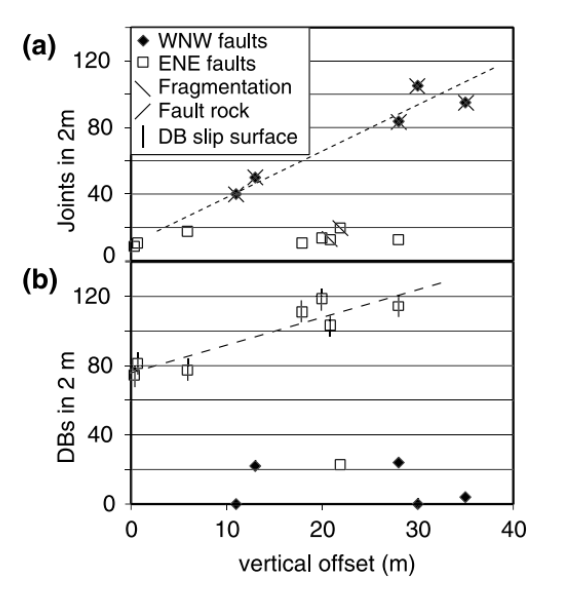
\includegraphics[scale=0.5\textwidth]{DavatzesFR}
    
%	\caption{ Vertical offset versus (a) number of joints and (b) number of
%deformation bands within 2 m of fault slip surface. Data were
%collected from different locations along single faults as well as
%several different faults. Associated structures such as fragmentation,
%deformation band slip surfaces, and fault rock related to joint-based
%faulting are also indicated. Depiction of  From Davatzes}

%	\label{fig:DavatzesFR}
	
%\end{wrapfigure}


In this study we refer to \textit{fault rock} as rock altered either mechanically or chemically by the influence of the fault. At all field locations we observe diverse fault rock lithologies, ranging from finegrained cataclasites to massive  bodies of breccias (up to meters of thickness). 

We suspect some fault rock associations exists. For instance, Davatzes et al., 2002 reports of a systematic association between the lithology and the orientation of the fault set. Namely, the orthorhombic fault set striking WNW has systematic association with fragmentation, ubiquitous fault rock; whereas the ENE fault set rather has slip surfaces cutting through deformation band clusters (see figure \ref{fig:DavatzesFR}}). This relations may the result of contrasting genetic mechanism. The WNW set is the result of the reactivation of regional joints. In contrast the ENE fault set is the the result of clustering and anastamosing deformation bands acting as a catalysing agent to the formation of a faults.

\subsubsection{Deformation Bands}

Deformations bands where a nearly ubiquitous feature of all fault structure in the the high porosity sandstones featured in this study. Deformation bands accommodate small amounts of deformation by the run-away collapse of grains in sub planar sheets--or bands (as seen in cross section). Around fault structures, deformation bands most often accomodate small (up to a few centimetres) of shear offset across thin (up to a centimetre thick) bands. Unlike slip surfaces these do not reduce the relative cohesion of the rock. It was not possible to crack them open. In zones of intense shear, deformation band clusters occur. The clusters are networks of anastamozing deformation bands.

By the reduction of grain size and compaction, deformation bands are relatively stronger than the host sandstone. Correspondingly, deformation bands preferential resist erosion and outcrop as slabs up to meters in sizes (especially in the Entrada Sandstone). The edge of the slabs is coated with a host sand grains. In cross section, deformation bands have a milky white colour and have a sinuous trace--moreso than than slip surfaces. Albeit, it is sometimes difficult to differentiate slip surfaces from deformation bands in cross-section. The edge of deformation band clusters appear to have a distinct "lumpy" morphology. Moreover, there is a clear directional asymmetry (see figure \ref{DBC})

Ultimately, given sufficiently intense deformation, it is thought that faults develop on one of the edges of the cluster. Presumably, the mechanically stronger properties of the deformation bands lead the concentration of stress around the clusters. Observations from this study do not necessarily agree with this paradigm. Deformation bands active after the onset of a stable slip surface \textit{have} been observed at Big Hole (Shipton and Cowie, 2003). These are presented as fault related damage. Onset of late deformation bands may reconcile our observations with the existing paradigm for fault development in high porosity sandstones. We intend to explore the surface roughness of the edge of deformation band clusters. In a sense, these surfaces could represent a 'primordial roughness'.

At some locations, take for instance the Blueberry Fault in the Chimney Rock Fault Array, deformations bands seems to be the overwhelming mechanism to accommodate off-fault damage. When considering issues of fault mismatch related to roughness and consecutive displacement, deformation bands may be an effective mechanism to accommodate inelastic fault perpendicular deformation.
 
 \begin{figure}[H]
	\centering
	\begin{subfigure}[b]{0.4\textwidth}
		\includegraphics[width=\textwidth]{DBC_edge}
	\end{subfigure}
	~
	\begin{subfigure}[b]{0.4\textwidth}
		\includegraphics[width=\textwidth]{DBC_X}
	\end{subfigure}
	\caption{Left: Example of the edge of a deformation bands cluster at Molly's Castle. Note the "lumpy" morphology and an clear vertical directional asymmetry. Right: Cross-sectional view of a deformation band cluster with tens of centimetres of shear offset. It is unclear weather there is a through going slip surface localizing displacement. It is , however, definitely not on the edge of the cluster.}
	\label{DBC}
\end{figure}		

\section{Model}
	\subsection{Model Outline}
	\subsection{Model Results}

\section{Discussion}
	\subsection{An external estimate of gouge production and fault thickness}

The data collected in this study offers the unique opportunity to provide new indirect estimates of fault rock production, fault thickness and dilation rate over an entire fault. We know that 1) the primordial roughness is systematically rougher than mature faults, 2) the primordial roughnes is relatively constant, and 3) the roughness can be estimated for a given displacement. Using these results, I will estimate the volume of fault rock produced through wear and the corresponding roughness induced accomodation space in the fault system.

Displacing two rough fractal surface in shear requires dilation. The expectation dilation can be estimated according to the amplitude of the largest wavelength ($\lambda$) being offset (see figure XXX). For a given displacement, $u$, the largest wavelength in the system will be $\lambda = 2u_i$. Using a fractal paradigm to define the average amplitude of a given wavelength according to the pre-factor $\Beta$ and the Hurst scaling exponent, $H$, (*reference the equation*) we find that the dilation, $A$ can be expressed as a function of displacement:

\begin{equation}
	A(u) = \sqrt{\Beta 2u^{-2H-1}}
\end{equation}

If we apply this to an entire fault system with displacement field, $U$, we can estimate the void space that would be produced:

\begin{equation}
	V_{void}(U) = \int_S \sqrt{\Beta 2U^{-2H-1}}dS
\end{equation}

Since the fault system is closed any change in fault roughness $must$ be coupled to the fault core. If all changes in the fault surface are associated to a production of fault rock, we can effectively estimate the volume of fault rock that has been produced from diplacement $u_0$ to $u_f$ by comparing the volume integral under the corresponding initial and final slip surfaces $S(u_0)$ and $S(u_f)$.

\begin{equation}
	\dfrac {\Delta V_{fault rock}}{\Delta u} = \int_S S(u_0) - S(u_f) dS
\end{equation}

volume integral under the surfaces, $S$, can be estimated numerically according to the frequency distribution prescribed by the RMS the  entire fault system. Note that the RMS is estimated at the length scale of the entire fault; wear processes are active at all length scales below this.

\begin{equation}
	\int S dS \approx 
\end{equation}

Now for the displacement field, $U$, we can estimate the total fault rock produced by using the primordial surface roughness, $S(0)$, and the prediction of the surface roughness extrapolated to the length of the fault (* reference the the equation of smoothing *) such that:

\begin{equation}
	V_{fault rock}(U) = \int_S S(0)-S(U)dS
\end{equation}

The comparison between the two quatities is telling. If the amount of fault rock is

\section{conclusion}

\section{Appendix}

\subsection{Surface Processing scripts}

Or possibly a link to a git repository...

\subsection{User manual for script}

\chardef\_=`_

This manual should serve as both a basic guide to the logic and usage of the \textit{surface processing package}. 

The master function of the package is \textit{surfaceprocessing}. This function effectively deal with the inputs and direct computations towards the necessary functions. Outputs of the function are a .mat workspace file for each input data file. The workspace includes a structure (called \textit{parameters}) with the raw surface analysis outputs, the point spacing, the decimation factor (if any), the file name and the date of the analysis. The workspace also includes the grid form of the original inputed surface (called \textit{surface}), and the pre-processed copy that was used for the subsequent analysis (called \textit{zGrid}).  Inputs are always included in pairs. The former defines the type of input, the latter qualifies or quantifies the input. This structure allows for adaptability of the code to various needs. Options include the following:

\begin{itemize}
\item \textit{what to do?}: 'toDo', followed by the desired analyses on of: 'FFT','PLOMB', 'parameters' or 'all' (default is 'all') - can be a cell array. This specifies what kind of spatial analysis will be done on the input surface data. The spatial analysis is calculated and averaged across every single profiles along the surface.  The analyses are the following:
	\begin{itemize}
	\item 'FFT', a power spectrum computed using a Fast Fourier Transform (FFT) algorithm; 
	\item 'PLOMB', a power spectrum computed using a least-squares Lomb-Scargle algorithm;
	\item 'paramters', the calculation (as a function of scale) of the Root Mean Squared (RMS), skewness, kurtosis and asymmetry averaged across all segments of a given length on all profiles of the surface.
	\end{itemize}

'all' simply performs all the analyses outlined above.

\item \textit{skip pre-processing?}: 'bypass', followed by 'zygo', 'pre-processing' or 'no' to  be used input is already in aligned clean grid form - input files are then (default is 'no'). 'zygo' is specifically adapted to the proprietary data format of the white light in Wong. 'pre-processing' simply skips any pre-processing. This option requires a .mat structure with a field named 'grid' with the topography and a field name 'pointSpacing' specifying the point spacing (in meters). In either case the topography must be aligned such that the positive x direction is the parallel direction.	

\item \textit{for the parameter analysis, how many scales?} 'numberOfScales' followed by the desired number of analysed scales. This option is relevant to the parameters analysis. Note that this has a lot of effect on the amount of processing time (default is 10).

\item \textit{decimation}: 'decimationFactor' followed by the desired decimation factor (default is 1). Decimation is a useful tool to reduce computation time. The surface grid is sub-sampled according to the decimation such that a decimation factor of $k$ would imply that only every $kth$ point on the every $kth$ will be considered for hte subsequent analysis.

\item \textit{Instrument specific analysis} 'instrument' followed by 'white light', 'laser scanner' or 'lidar' (default does not set any instrument specific adjustments). Some instrument specific pre-processing steps are taken. Please contact me if you intend to use this as they may be highly dependent on the specific instrument used.
	 
\end{itemize}

For instance, \textit{surfaceprocessing('todo','FFT','bypass','zygo')} will only perform a power spectral density analysis and will skip preprocessing and assume that all input will be in the 'zygo' export .xyz format.

When the command is executed, the user will be prompted to navigate to the directory where the input data is located. IMPORTANT: the directory must \textit{only} contain files of one data format. There cannot be other files or sub-directories in the directory. The user will then be prompted to choose a destination for the output data. The requirements for the output location are less stringent. However, it is advisable to choose an empty directory such as to facilitate subsequent steps.

The next step is to visualize the output of the analysis. This is done using the \textit{unpack parameters} function. This function provides various visualization options for all files in the directory chosen by the user. The first input (the \textit{desired plot}) can be one of the following:

\begin{itemize}
\item[] \textit{'FFT'}: plot all power spectra;
\item[] \textit{'PLOMB'}: periodogram plot as determined by the Lomb-Scargle least squares analysis;
\item[] \textit{'topostd'}: plot of the root mean squared (RMS) as a function of scale;
\item[] \textit{'topoSkew'}: plot of skewness of height fields as a function of segment scale;
\item[] \textit{'topoKurt'}: plot of the the kurtoisis of height fields as a function of segment scale;
\item[] \textit{'PowerVsDisp'}: plot of power interpolated at a given scale as a function of displacement;
\item[] \textit{'RMSVsDisp'}: model RMS at a given scale as a function of displacement
\item[] 'Grids': shows both the original and pre-processed grid for the specified file 'fileName';
\item[] \textit{'Best Fits'}: best logarithmic fits to power spectra obtained from the fast fourrier transform analysis.
\end{itemize}

The functionality of the packages is broadly divided into three sections: 1) importing and preprocessing data, 2) performing various spatial statistics on the pre-processed data, and 3) unpacking the analysis output into figures.

In order to run smoothly the all functions included in the package should be kept in the same directory or on an accessible path. 

For reference, here is a quick outline of what each function does:

\begin{itemize}
	\item[] \textit{affine\_fit}: (from mathworks) Computes the plane of best fit using least squares normal distance;
	\item[] \textit{align\_grid}: finds the smoothest directions in a grid using FFT spectra and rotates and re-grids the input grid;
	\item[] \textit{fault\_spectral\_density\_simple}: Calculates the average lomb-scargle spectral density every row of a N by M array;
	\item[] \textit{FindErr\_loop\_anisotropy}
	\item[] \textit{flatten\_XYZ}: removes planar trends from XYZ data by applying a rotations matrix according to the best fit plane (affine\_fit);
	\item[] \textit{fractal\_model\_outlier}: Removes outlying segments according to a near-gaussian model for the distribution of RMS values at specified segment lengths (or scales);
	\item[] \textit{frequency\_spectrum}:Calculates the average lomb-scargle spectral density of all continuous 	segments on every single row of a N by M array;
	\item[] \textit{parse\_zygo\_format}: extracts the both the point spacing and topographic grid from the exported zygo format. Can also remove planar trend from data (substracted from grid);
	\item[] \textit{rotateZ}: applies rotation matrix on XYZ data
	\item[] \textit{surface\_analysis}: Aggregates the analysis functions and applies them to an input grid
	\item[] \textit{surface\_cleaning}: removes outliers associated to surface defects
	\item[] surface\_parameters: calculates spatial statistics and parameters along segments as a function of scale (RMS, skewness, directional asymmetry and kurtosis)
	\item[] \textit{surface\_preprocessing\_2}: deals with preprocessing input data (import data, cleaning and gridding data)

\end{itemize}


\end{document}
